\subsection{Experimental Setup}\label{subsec:experimental-setup}
%
%推定したい真のvelocity modelは101 x 51のgrid pointsで構成されます.
%初期velocity modelは、真のvelocity modelを標準偏差は80のガウス関数で平滑化したものを使用します.
%source waveletは10 Hzの主周波数を持つRicker waveletを使用します.
%shot数とreceiver数はそれぞれ101と20です.
%勾配Eの計算はdevitoを用いて行われました.
%
%the velocity model is composed of 101 and 51 grid points in the horizontal and vertical directions, respectively.
%We use source wavelet that a Ricker wavelet with a dominant frequency of 10 Hz as the source wavelet.
%number of shots and the receivers are 101 and 20, respectively.
%the initial model obtained by smoothing the velocity model with a Gaussian smoothed function where the standard deviation is 80.
%
To demonstrate the effectiveness of the TV and box constrained FWI, we conducted experiments where we compared with the normal FWI with gradient method, using the SEG/EAGE Salt and Overthrust Models.
The velocity model consists of 101 $\times$ 51 grid points, and the initial velocity model is generated by smoothing the true velocity model with a Gaussian function with a standard deviation of 80.
Number of receivers and source shots are 101 and 20, respectively.
The source wavelet is a Ricker wavelet with a central frequency of 10 Hz.
The gradient of $E$ is computed using the Devito framework\cite{devito}.
In normal FWI, the step size is set to $1.0 \times 10^{-4}$.
In TV and box constrained FWI, the step size $\gamma_1$ and $\gamma_2$ are set to $1.0 \times 10^{-4}$ and $1.0 \times 10^2$, respectively, the upper bound of the $l_{1,2}$ norm $\alpha$ is set to 400 and the lower and upper bounds of the velocity model $a$, $b$ are set to 1.5[km/s] and 4.5[km/s], respectively.




\subsection{Results and Discussion}\label{subsec:results-and-discussion}
%Table 1 presents a summary of the restoration performance achieved by DnCNN-PnP-PDS and other methods. Across all tasks, we rec- ognize that our proposed DnCNN-PnP-PDS has achieved restoration performance comparable to that of DnCNN-PnP-FBS. We remark again that the proposed approach simplified parameter tuning when compared to DnCNN-PnP-FBS. Specifically, in this experiment, we √ rewrite the parameter ε in (9) by α ∈ R as follows: ε = ασ K. √ Note that σ sian noise with the variance σ. The value of α in DnCNN-PnP-PDS was set to 0.95 for all cases, whereas λ in (10) varied from task to task for DnCNN-PnP-FBS. Additionally, we experimentally found that in deblurring, the appropriate λ value was higher than in inpainting. Therefore, in deblurring with a low σ value of 0.005, DnCNN-PnP-PDS achieved a higher PSNR value by approximately 2.5 [dB] compared to
%DnCNN-PnP-FBS. This result supports the versatility of the de- noiser discussed in Section 3.3. Furthermore, the methods with DnCNN consistently led to sta- ble restoration in all tasks, while the methods with BM3D resulted in instability and cases where restoration did not proceed properly, as seen in the inpainting scenarios. Two possible reasons for this result can be considered: 1) BM3D is generally not firmly nonexpansive, leading to a lack of theoretical guarantees. 2) BM3D assumes the presence of many similar structures within the image [11, 15]. How- ever, this assumption did not hold in images with numerous random missing regions, leading to a significant decrease in restoration per- formance. In Fig.1, we present cn and PSNR values for each iteration. We observe that cn converges to 0 in both cases of DnCNN-PnP- FBS and DnCNN-PnP-PDS. This stability was achieved due to the firm nonexpansiveness of the denoiser. The visual results in Fig.2 show that the clean output of DnCNN-PnP-PDS. In the TV case, color irregularities were observed around the yellow rope, and in the BM3D-PnP-FBS, BM3D-PnP-PDS, and DnCNN-PnP-FBS cases, the images became overly smoothed, resulting in the loss of fine de- tails in the floor pattern. In contrast, DnCNN-PnP-PDS successfully restored the features of the rope clearly, leading to sharp results.


\begin{figure}[htbp]\label{fig:ssim}
%\vspace{-\baselineskip}
\begin{center}
    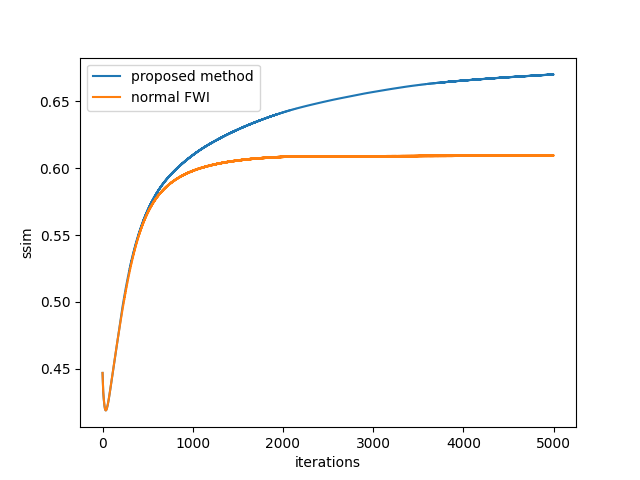
\includegraphics[width=80mm]{public/ssim}
    \caption{ssim}
\end{center}
%\vspace{-\baselineskip}
\end{figure}
